\chapter{Literature Review} \label{chap:litreview}

\bigskip
\section{The Beginning of the Web, the Birth of WebAssembly}

The Internet, specifically the World Wide Web standards \cite{lit1}, is a set of protocols behind every modern web browser. With the internet, we have the access to recourses, documents, and books that even the most powerful people just a few decades ago could not have dreamt of. With the internet, we can achieve incredible things.

In 2017, a new World Wide Web standard was developed and integrated with most of the modern web browsers, named WebAssembly (WASM) \cite{lit2}. When the technology was first developed, it was designed to enable users to run large-scale desktop applications straight from their web browsers, while keeping the applications’ high-performance nature. Thus, it helped to solve some of the most critical issues that impact traditional software. For example, the issue of backward compatibility with newer software updates - when developers release new versions of their software, they may want to make changes to the user interface or the behavioural logic by adding new features or removing unwanted existing features. Traditionally, the solution to this is to issue a software update – users will be asked to download and reinstall the software for the latest features and user experience. However, this is a moderately complicated process, and it would be unpopular amongst users if the updates are issued too regularly. Thus, only a small percentage of all users manually update their software regularly. According to the study done by Moller et al. \cite{lit3}, on average, only 17 per cent of all users install updates from the Apple App Store \cite{lit4} or Google Play Store \cite{lit5} on the day of release. And only about half of all users choose to update their app after a week of release.

\newpage
\bigskip
\begin{figure}[hp]
\centering
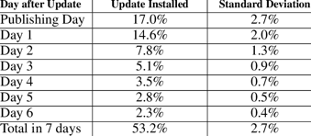
\includegraphics[scale=0.75]{litr1}
\caption{\footnotesize{Percentage of users updated within 7 days following a release \cite{lit3}}}
\captionsetup{aboveskip=0pt,font=it}
\end{figure}
\bigskip

Problems like this are what motivate engineers and industry experts to develop solutions and workarounds. After years of discussions and meetings from universities, major tech companies and research institutions, the concept of WebAssembly was born. And a few years after that, the language itself was developed and ready to be shipped.

\bigskip
\section{Security Vulnerability}

One of the main reasons that major PaaS (Platform as a Service) companies use virtual machines and containers to host their clients’ applications is security. As stated above, both VM-based and container-based deployment approaches have the ability to limit the exposure of system APIs, which protects the physical hardware’s operating system from malicious code. However, on top of that, quite a few other software features that we use every day might also introduce vulnerabilities.

One example is that in order to improve the user experience on regular software updates, companies and developers have introduced a relatively more convenient way to manage software updates – automatic updates. For example, Google Chrome powered by Chromium has the auto-update feature turned on by default \cite{lit6}, Apple also has a similar feature with their iOS App Store with an option to turn off auto-updates \cite{lit7}. The main benefit of auto-update is that it always keeps the software up to date. However, researchers have shown that auto-update can introduce unwanted side effects. Geer (2021) argues that by adding an auto-update feature to the software, not only it is making the software more complex with more potential to introduce errors and bugs in the future. More importantly, the software developer is giving something to their users regardless of whether the user would want the updates or not \cite{lit8}.

Geer believes that this would give the software developer too much control over their users. Further, Geer stated that when software has an auto-update feature, the developers are more likely to feel pressured to push out new updates periodically, thus more likely to produce lower quality code as well as design structures. This has the potential to introduce unexpected or unwanted bugs into the code and therefore cause unexpected issues to the software itself. Luettmann (2007) argues that the fundamental issue with auto-update is that there are currently no established standards or institutions to address such an issue \cite{lit9}. Luettmann also stated a few other potential security issues regarding software auto-update. In their research, Luettmann presented the “man-in-the-middle” (MIMT) attack. A popular way to carry out a MIMT attack is a proxy attack. This is usually performed by hijacking a middleware service or a proxy server between the user’s client machine and the target server machine. Thus, sending out data packets with fraudulent information and potentially installing spyware or malware on the end user’s computer. The other way to perform a MIMT attack is to intercept the communication between the user’s devices to an unsecured LAN local network, also known as an injection attack. Injection attacks are usually easier to perform since this method is taking advantage of unsecured networks. This usually occurs on public Wi-Fi networks such as cafés and restaurants which are usually more vulnerable than password-protected networks if not set up correctly.

\bigskip
\begin{figure}[hp]
\centering
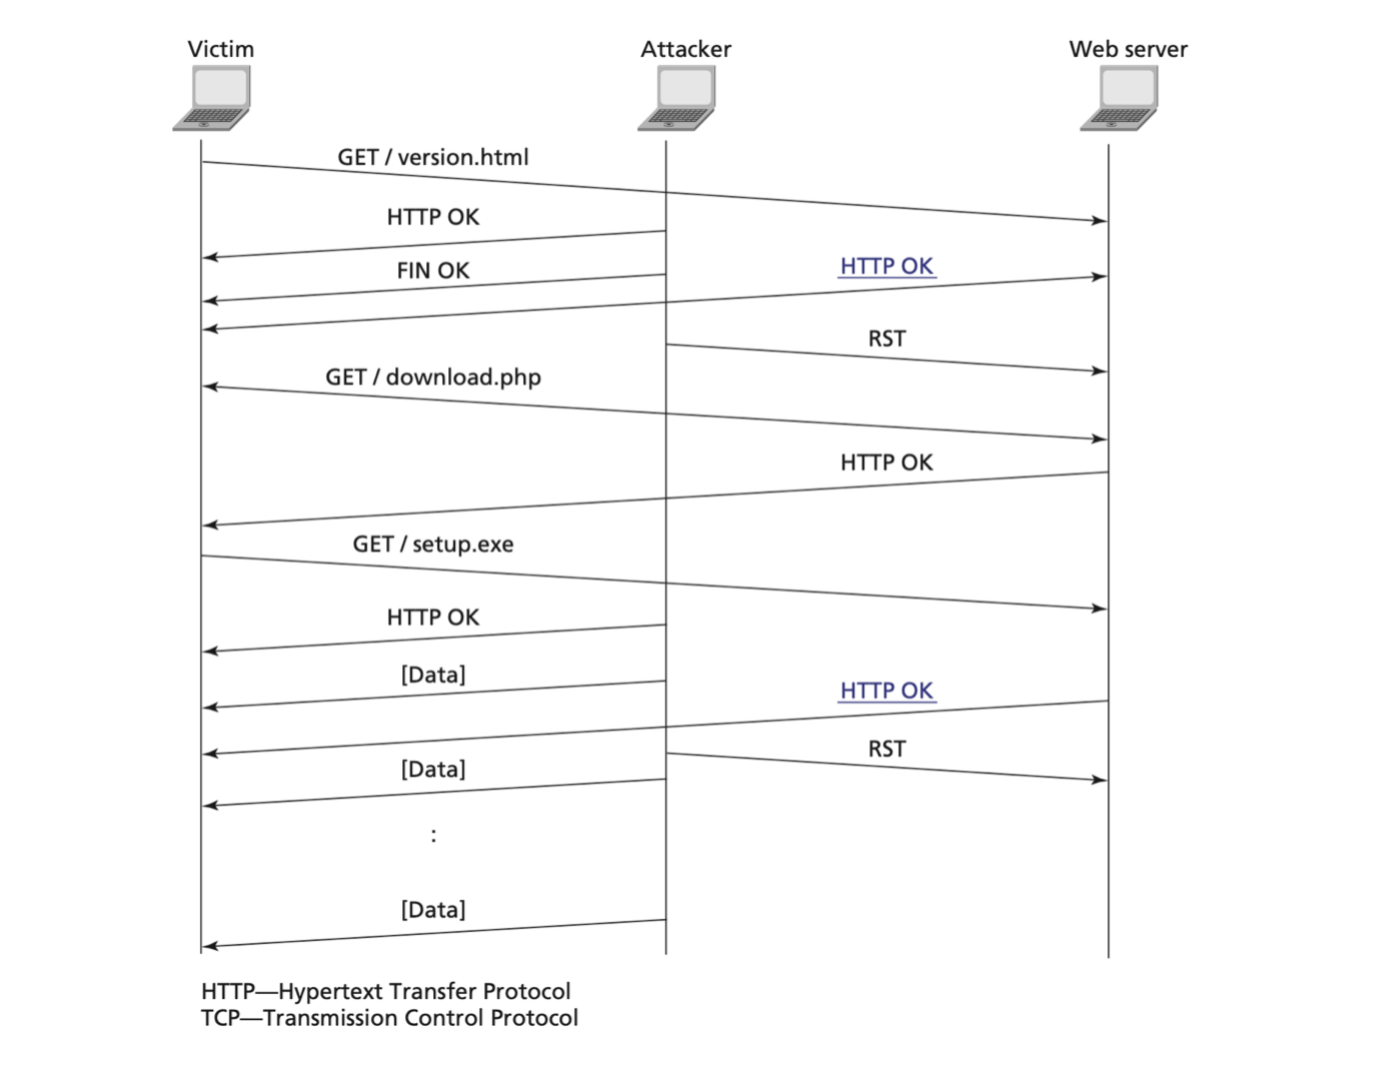
\includegraphics[scale=0.8]{litr2}
\caption{\footnotesize{A MIMT attack \cite{lit9}}}
\captionsetup{aboveskip=0pt,font=it}
\end{figure}
\bigskip

Luettmann looked at a few software by examining the communication packets and files between the client software and the server computer. Including Adobe Acrobat, Microsoft Windows XP, Zango, and Cam2PC. From their research, they identified Adobe Acrobat and Microsoft Windows XP to be relatively secure when it comes to issuing auto-updates. However, Zango and Cam2PC were found to be potentially vulnerable to MIMT attacks. The authors believe that the reason Adobe Acrobat and Microsoft Windows XP are more secure with auto-update is that both software used a method called “code signing”. With this method, the device receiving the update would be able to verify the legitimacy of the owner as the data packet sender, thus making sure that the update packet will always be coming from a verified software distributor. However, Luettmann stated that even with proper data verification features in place, it does not necessarily mean that there will be no issues with the updated software. Luettmann emphasises that writing and delivering issue-free/bug-free programs are just as important as all the security features built into auto-update. On the other hand, Zango and Cam2PC are both to be found vulnerable to MIMT attacks as they do not have the “code signing” feature implemented. Lastly, much like Geer, Luettmann questioned if auto-updates were a good idea from the beginning, with auto-update enabled, the users would not be able to know when an update is occurring and thus will be vulnerable in certain circumstances. For example, when using an unsecured public Wi-Fi.

\bigskip
\begin{figure}[hp]
\centering
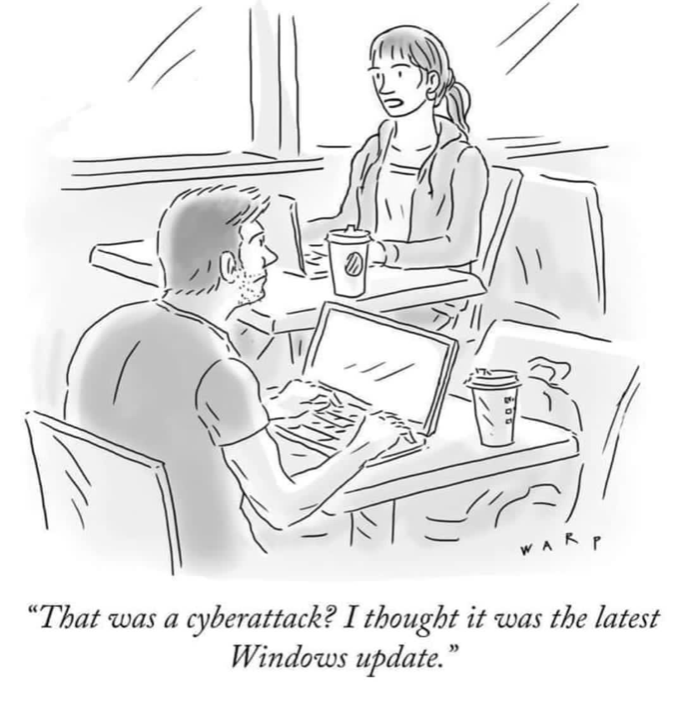
\includegraphics[scale=0.8]{litr3}
\caption{\footnotesize{An online meme post in regard to internet security breaches \cite{lit10}}}
\captionsetup{aboveskip=0pt,font=it}
\end{figure}
\bigskip

\bigskip
\section{Safety with WebAssembly}

The auto-update issue stated above is just one of a dozen issues desktop application developers must consider when developing new applications. Rossberg et al. (2017) presented and showcased the whole concept of WebAssembly. This includes the design motivation, the properties, the benefits of using WebAssembly as well as the fundamental maths and code concepts behind WebAssembly \cite{lit11}. In the article, the authors first acknowledged that WebAssembly is safe, fast, portable, and efficient. Then, they listed several benefits of developing applications using WebAssembly. After that, the authors introduced the fundamental design concepts and design pathways engineers and developers undertook when developing WASM, as well as some of the maths correlated with those concepts. Lastly, the authors undertook discussions about edge cases, compliers, and future/related works.

Rossberg et al. listed several benefits of WebAssembly. Firstly, its safety features – during the development of WebAssembly, developers and researchers were partially inspired by the “sandbox” technology used on mobile web browsers. Web browsers running on mobile operating systems such as Apple's iOS and Google's Android can run external code from a virtual machine, thus preventing malicious code from trying to compromise physical devices. Secondly, its speed – As stated in the introduction, instead of writing WebAssembly code directly, WASM applications are written in traditional languages such as C, C++, or Rust, after that, they will then be compiled down to WebAssembly through a WASM runtime. There are plenty of WebAssembly runtimes to choose from, and most of them have the ability to utilise full system performance in order to speed up the application to a near-native performance \cite{lit12}.

\bigskip
\begin{figure}[hp]
\centering
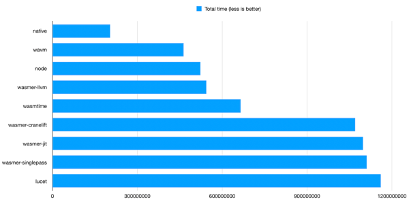
\includegraphics[scale=0.9]{litr4}
\caption{\footnotesize{Performance of different WASM runtimes compared to native runtime \cite{lit12}}}
\captionsetup{aboveskip=0pt,font=it}
\end{figure}
\bigskip

\bigskip
\section{Compatibility and Speed}

On top of that, WebAssembly also have the benefits of being universal and portable – not only WebAssembly is a brand-new technology, but it is also a fully integrated W3C standard. This means that WebAssembly runtimes, including all its core functions, will be available to run on every modern web browser alongside JavaScript runtimes. This can be critical for the wide adoption of the technology because WebAssembly will no longer be “just another tool trick” that can only be used in a few specialised browsers, but in all browsers that support the latest W3C standards. This way, WebAssembly can run on most devices and operating systems, making it as universal as JavaScript itself. Lastly, since WebAssembly can be compiled down to raw binary code, which is a lot more compact than JavaScript files, those binary files can be transferred faster between servers and clients’ computers, which has the potential to increase website loading time.

However, despite all the benefits we’ve seen from WebAssembly, WASM was never intended to replace JavaScript. Instead, it was designed to be running alongside JavaScript and to handle specific high-performance applications to increase the potential of web browsers. However, some tools and frameworks exist on the market that allows users to build entire websites with WebAssembly, namely Microsoft’s Blazor framework \cite{lit13}.

Reiser and Bläser (2017) presented Speedy.js, a cross-compiler engine that can compile JavaScript/TypeScript code to WebAssembly \cite{lit14}. Speedy.js allows users to write entire web applications in JavaScript/TypeScript and to be compiled down to WebAssembly code before running in a browser, according to Reiser and Bläser, JavaScript/TypeScript compiled to WebAssembly can accelerate the code up to four times faster than running the code natively.

\bigskip
\begin{figure}[hp]
\centering
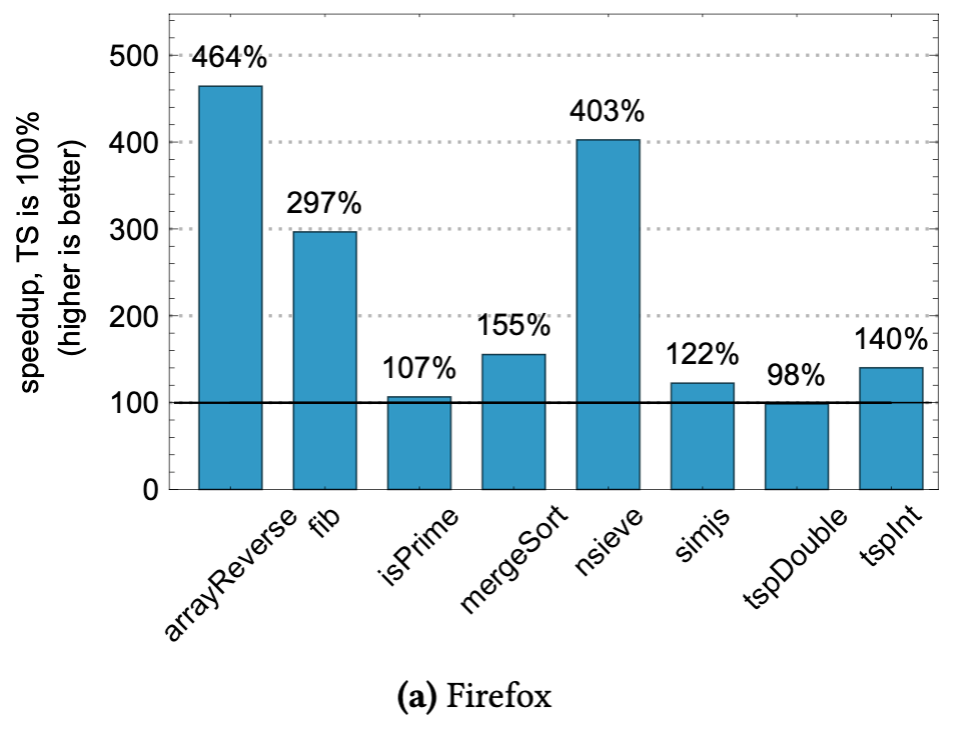
\includegraphics[scale=0.7]{litr5}
\captionsetup{aboveskip=0pt,font=it}
\end{figure}
\bigskip

\newpage
\bigskip
\begin{figure}[hp]
\centering
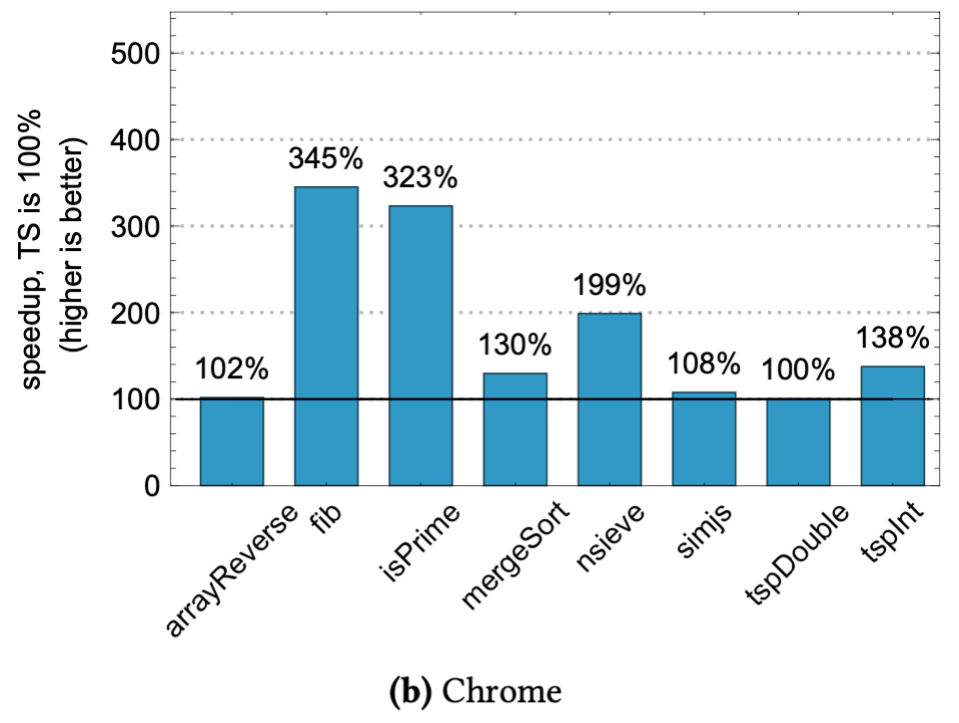
\includegraphics[scale=0.7]{Picture6}
\caption{\footnotesize{Performance of Speedy.js compiled code compared to JavaScript/TypeScript code running natively in two web browsers: Mozilla Firefox (a), and Google Chrome (b) \cite{lit14}}}
\captionsetup{aboveskip=0pt,font=it}
\end{figure}
\bigskip

Reiser and Bläser undertook an experiment comparing the performance differences between native JavaScript/TypeScript code and WebAssembly code that was compiled from Speedy.js running in two modern web browsers – Mozilla Firefox and Google Chrome on eight test cases. That is: 1 - reverse an array; 2 - calculate the Fibonacci number of 40, 3 – test if a number is prime, 4 – merge sort an array, 5 – calculate the number of prime numbers in a range using the sieve of Eratosthenes, 6 – using the SIM.js library to generate a thousand random numbers, and finally 7 and 8 – the travelling salesman problem. The above figure shows that after running all the test cases in both web browsers, WebAssembly code has a significantly faster runtime than running JavaScript/TypeScript code natively on all tasks except for one. More importantly, the authors stated that in order to use Speed.js to compile native JavaScript/TypeScript code into WebAssembly code, only minimal changes need to be made to the native code. Thus, it is able to make itself more attractive to developers that would like to experience this technology.

During the performance experiments, Reiser and Bläser discovered that after removing some of JavaScript’s safety checks, they observed an increase in the web application’s performance. Hence, they proposed that it might be a good idea for browser developers to investigate adding support to JavaScript code with a relaxed set of safety guarantees in order to increase the performance for some of the more complex web applications.

A few years before Reiser and Bläser conducted their research, Herman et al. from Mozilla developed asm.js \cite{lit15}. It was released in 2014 and it was one of the first pieces of software that were developed with the concept of running non-JavaScript code in web browsers.

According to Herman et al., Asm.js is a “strict subset” of JavaScript and it has the ability to compile and execute memory unsafe languages such as C or C++ in a sandbox environment before running them in web browsers.

The concept of asm.js is similar to speedy.js. Both programs compile and “translate” the language used during development to a different language to be used in the compiled software. However, compare to speedy.js, asm.js behaves more aligned with the concept of WebAssembly.

\bigskip
\section{The Problems with WebAssembly}

It is widely acknowledged within the WebAssembly community that compares to native code, WASM code is still lacking performance. Ever since the release of WebAssembly, researchers have been comparing the performance of applications running on web browsers using WebAssembly with applications running natively on native operating systems. There has also been a large amount of research and development work undertaken with the hope of increasing the performance of WebAssembly runtimes.

\bigskip
\subsection{JavaScript vs. WebAssembly Websites}

One of the most comprehensive studies on this topic was conducted by Yan et al. (2021). Yan et al. performed a systematic study in order to compare the performance between Native JavaScript code and the compiled WebAssembly code on 41 programs \cite{lit16}. The authors achieved this by first transforming all the programs’ C source code, compiling each program into both JavaScript code and WebAssembly code. They then deployed the programs alongside runtimes to different web browsers. Finally, the programs were run, and data were collected.

\bigskip
\begin{figure}[hp]
\centering
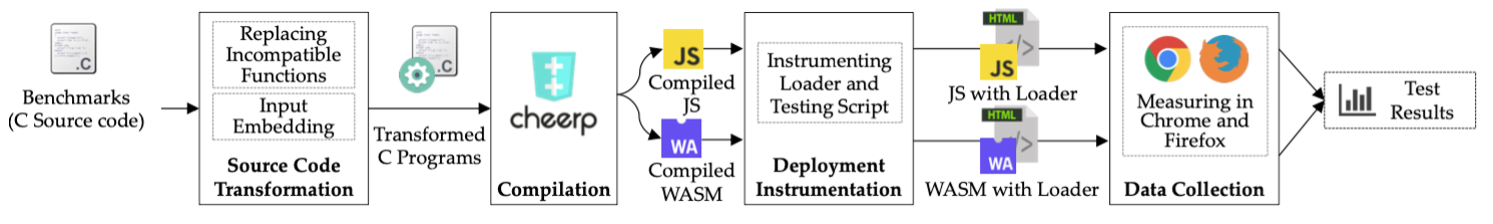
\includegraphics[scale=1]{litr7}
\caption{\footnotesize{The process of compiling C benchmark source code to JavaScript and WebAssembly code and running them in the Chrome and Firefox browser \cite{lit16}}}
\captionsetup{aboveskip=0pt,font=it}
\end{figure}
\bigskip

After running all the tests and collecting the appropriate data, the authors made several interesting discoveries. The authors found that not only WebAssembly’s just-in-time (JIT) compilers are not yet as efficient as their counterparts made for JavaScript, but they also found that WebAssembly uses considerably more memory than JavaScript code. The authors believe that this is because the JavaScript browser compilers have been continuously and thoroughly researched, developed, and tested for years while WebAssembly compilers are a relatively new concept. For example, JavaScript has automatic garbage collection to make sure memory usage is always kept within the appropriate range. However, WebAssembly currently lacks this feature. Furthermore, the authors suggested that more work is needed to optimise WebAssembly code execution. Yan et al. believe that as time moves on, JIT compilers for WebAssembly will be able to increase their performance significantly also widening its adoption within the industry.

When analysing the collected data, the authors observed a dramatic decrease in WebAssembly code’s runtime performance when the data input size increases. In fact, when testing using Google Chrome, WebAssembly is 27 times and 8.2 times faster than JavaScript when the input sizes are extra-small (XS) or small (S) respectively. However, as soon as the input sizes increased to medium (M), WebAssembly is only 2.3 times faster than JavaScript. Some programs, for example, the benchmark program “Lu”, were 62.5 times and 2.8 times faster than JavaScript when the input size is XS and S respectively. But suddenly slowed down to as much as 2.5 times slower than JavaScript when the input size increased to M. From here, the performance of WebAssembly only further decreased. When the input sizes are large (L) and extra-large (XL), WebAssembly on average only runs about 1.4 times and 1.6 times faster than JavaScript respectively with some benchmark programs running significantly slower than their JavaScript counterparts. Each program categorises the size of its input data differently, in-depth data can be found here \cite{lit17}.

\newpage
\bigskip
\begin{figure}[hp]
\centering
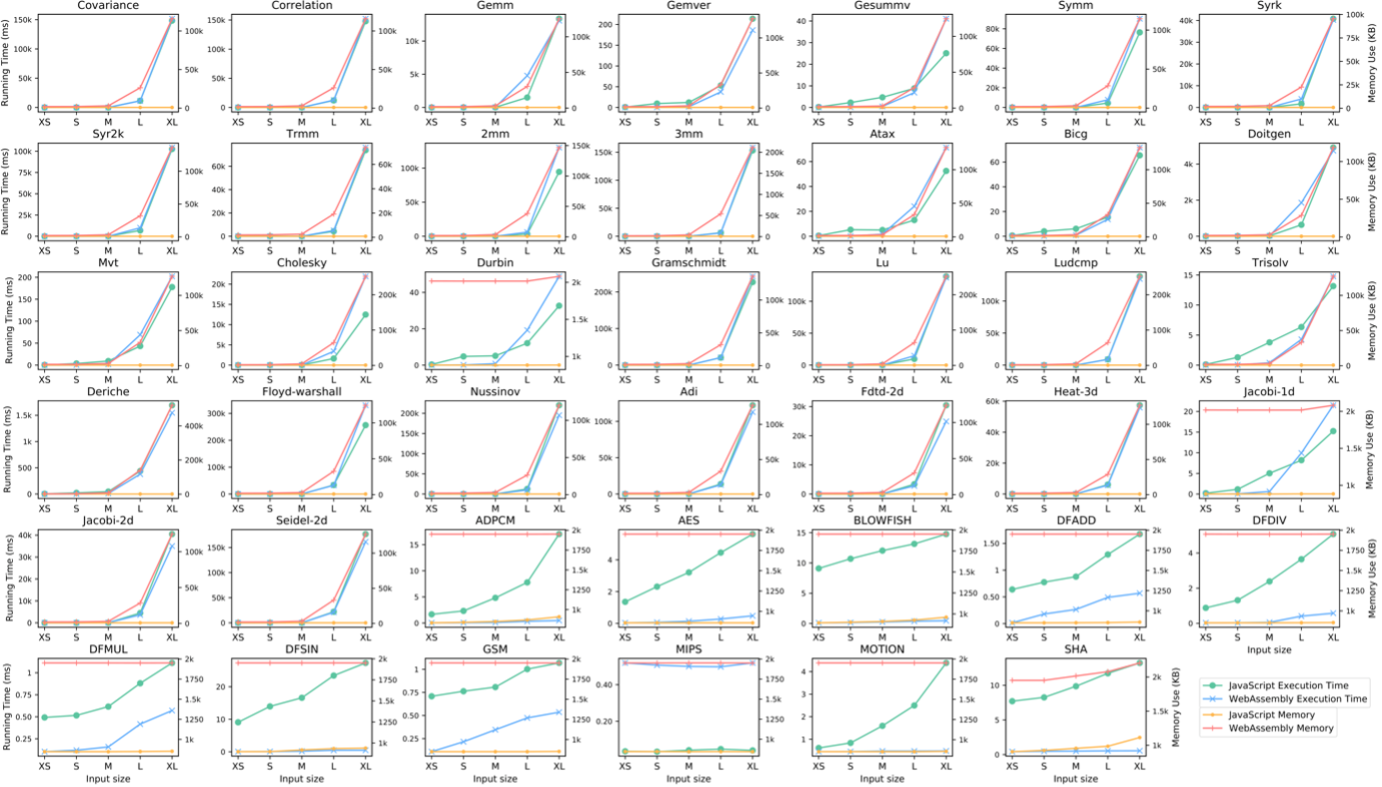
\includegraphics[scale=1]{litr8}
\caption{\footnotesize{Running all 41 benchmark programs’ C source code using WebAssembly and JavaScript. The left y-axis displays the execution time, and the right y-axis displays the memory usage \cite{lit17}}}
\captionsetup{aboveskip=0pt,font=it}
\end{figure}
\bigskip

After the experiment, the conclusion and justification from the authors are straightforward – JavaScript has been the “de facto” programming language for web development ever since its creation and initial release back in 1995 \cite{lit18}. In contrast to that, WebAssembly is a relatively new technology \cite{lit19}. The authors concluded that WebAssembly will be more developed in the future with more research and development undertaken.

\bigskip
\subsection{Unix vs. WebAssembly Desktop Applications}

Another challenge involved in the wide adoption of WebAssembly is its performance compared to applications running on native operating systems. An in-depth investigation was conducted by Jangda et al. (2019) \cite{lit20}. The team developed BROWSIX-WASM, which is an extension for Browsix – a framework that enables users to run Unix code in their browser \cite{lit21}. BROWSIX-WASM allows users to compile and run Unix programs that usually run in native operating systems to also run in web browsers.

Just like Yan et al., Jangda et al. compared the performance of several PolyBenchC benchmark programs and SPEC CPU benchmark programs between the two. The authors ran those programs on both Chrome and Firefox browsers as well as natively in the operating systems. The theory and hypothesis before experimenting was that generally, the programs running natively will have a stronger performance than the programs running on the browsers.

\bigskip
\begin{figure}[hp]
\centering
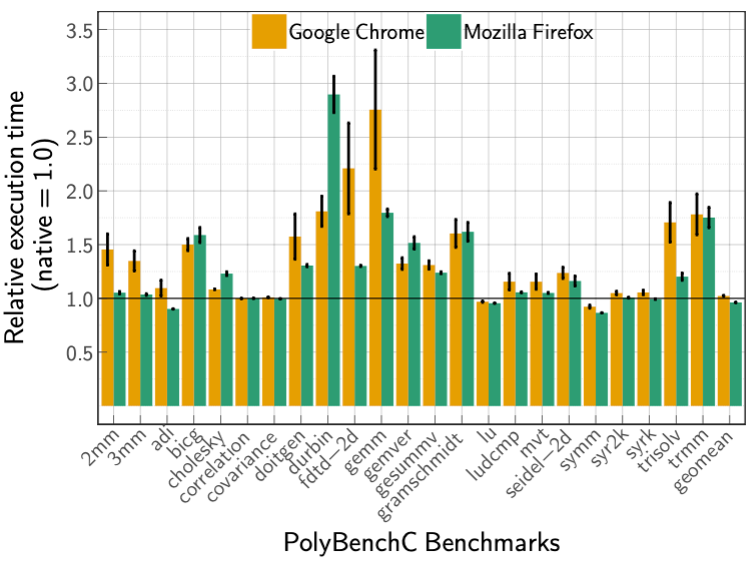
\includegraphics[scale=0.8]{litr9}
\captionsetup{aboveskip=0pt,font=it}
\end{figure}

\begin{figure}[hp]
\centering
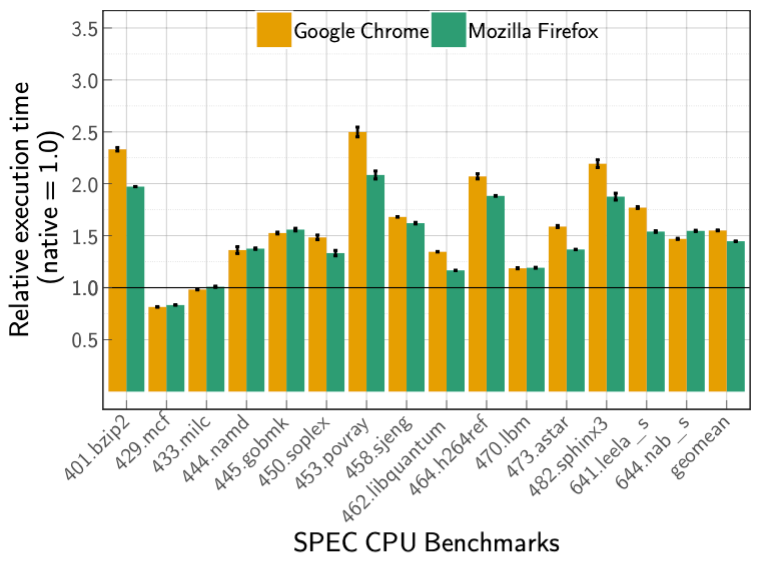
\includegraphics[scale=0.8]{litr10}
\caption{\footnotesize{Jangda et al. performing PolyBenchC and SPEC CPU benchmark tests with WebAssembly and native applications on Google Chrome and Mozilla Firefox \cite{lit20}}}
\captionsetup{aboveskip=0pt,font=it}
\end{figure}
\bigskip

After running the benchmark programs, the authors solidified their initial speculation. They observed that for almost all programs, WebAssembly performed worse than native applications. On average, WebAssembly was 1.55 times and 1.45 times slower than native applications when running on Chrome and Firefox respectively. It also had a peak slowdown of 2.5 times and 2.08 times on Chrome and Firefox respectively compared to native applications.

The conclusion formed by Jangda et al. is vastly similar to that of Yan et al.. They both suggested that compare to WebAssembly, JavaScript had a considerable head start as well as been in use for many years before WebAssembly was created. It has therefore received a lot more development and is also optimised for different scenarios. Lastly, Jangda et al. identified and made several pieces of advice and suggestions that have the potential to improve the performance of WebAssembly and its runtimes.

\bigskip
\section{Away from the browser}

It is not difficult to see why most people think WebAssembly is a technology that is only used on the web. To be fair, the word “web” is indeed in “WebAssembly”. However, from the very beginning during the design phase of WebAssembly, researchers and engineers have designed it to be a language that can run outside of web browsers. Similar to Node.js \cite{lit22}, WebAssembly is able to run as standalone applications in all operating systems with the help of WebAssembly runtimes such as aWsm and Wasmer \cite{lit23} \cite{lit24}.

Recently, there has been a growing interest in running WebAssembly applications on the Internet of Things (IoT) as well as edge devices. A number of researchers have worked on and built different software that run WebAssembly code outside of just web browsers. Wen and Weber (2020) proposed and developed an operating system that runs WASM code natively, called Wasmashine \cite{lit25} \cite{lit26}. The authors were able to achieve this by implementing a WebAssembly system interface (WASI) into the operating system in order to achieve communications between higher-level WebAssembly code and the underlying system kernel.

\bigskip
\begin{figure}[hp]
\centering
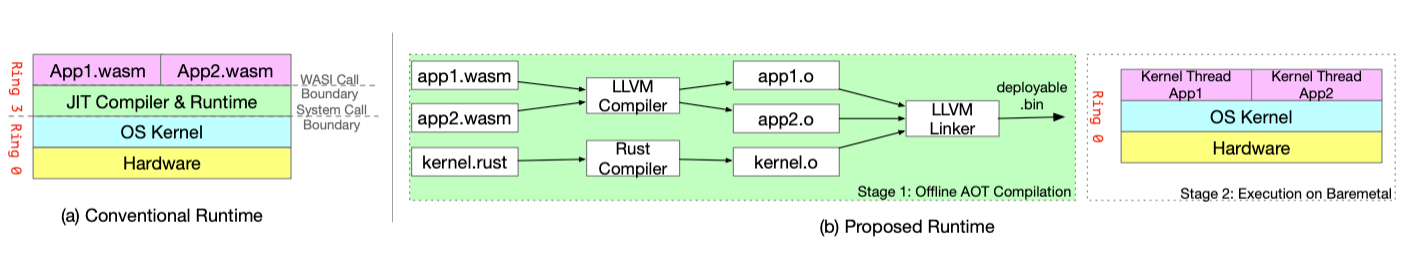
\includegraphics[scale=1]{litr11}
\caption{\footnotesize{The architecture of Wasmashine \cite{lit25}}}
\captionsetup{aboveskip=0pt,font=it}
\end{figure}
\bigskip

After the development of Wasmashine OS, the authors then installed it on a number of IoT and edge hardware devices such as Raspberry Pi microcomputers. Compared to the current model, they were able to achieve a faster program execution time when running programs in containers on these devices.

Eriksson and Grunditz (2021) configured a number of WebAssembly programs into containers and performed a comparison between WASM containers and Docker containers running on IoT/edge devices \cite{lit27}. The authors undertook testings using multiple WebAssembly runtimes. For example, Wasmer and Wasmtime. They also used PolybenchC benchmarking tool which is one of the most popular benchmarking libraries.

\bigskip
\begin{figure}[hp]
\centering
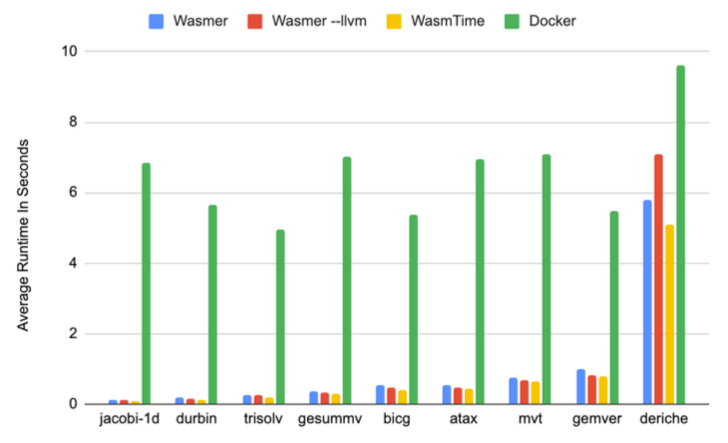
\includegraphics[scale=0.8]{litr12}
\captionsetup{aboveskip=0pt,font=it}
\end{figure}

\begin{figure}[hp]
\centering
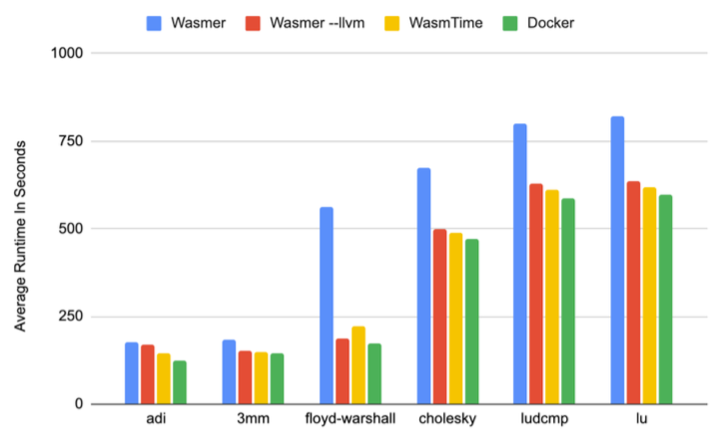
\includegraphics[scale=0.8]{litr13}
\caption{\footnotesize{Average low time-complexity and high time-complexity program runtimes \cite{lit27}}}
\captionsetup{aboveskip=0pt,font=it}
\end{figure}
\bigskip

From looking at the test result, we can observe that WebAssembly runtimes achieved a faster execution time than Docker applications on programs with low time complexity \cite{lit28}. However, when it comes to programs with a medium/high time complexity, those running with Docker containers scored the fastest execution time out of all the runtimes. This is very interesting as this result largely aligns with the results presented by Yan et al. (2021) which we reviewed earlier.

On top of that, another experiment with similar conclusions was performed by Napieralla (2020) \cite{lit29}. Napieralla’s research confirms that WebAssembly runtime containers outperform Docker containers consistently on application start-up times. But they also discovered that WASM runtime containers take longer to perform Read and Write I/O commands than Docker containers.

\bigskip
\begin{figure}[hp]
\centering
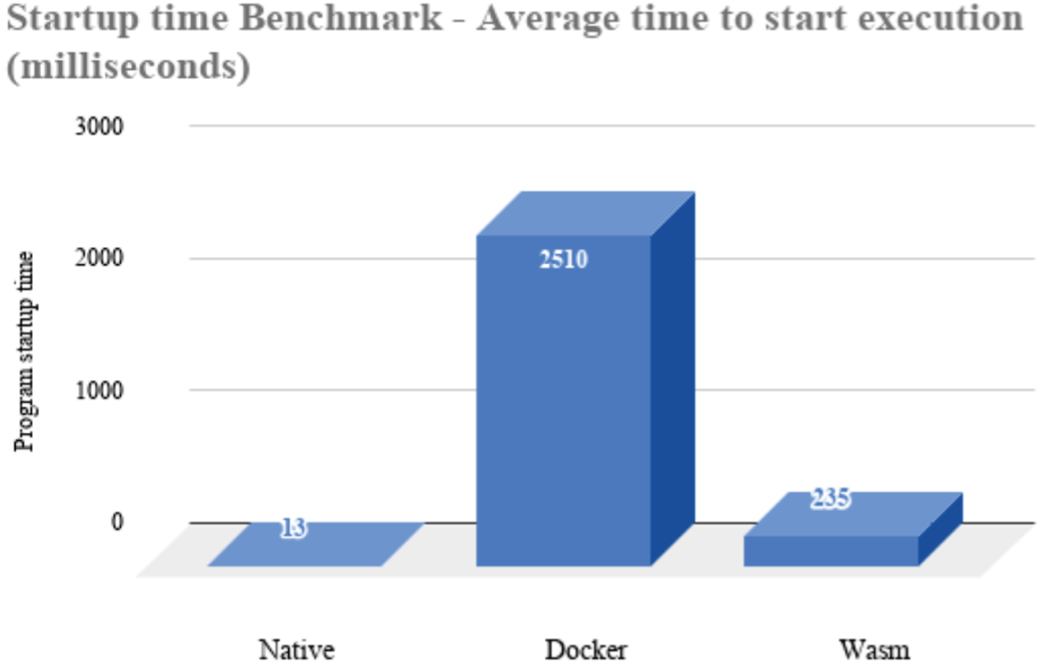
\includegraphics[scale=1]{litr14}
\caption{\footnotesize{Average start-up time between WebAssembly, Docker and Native applications \cite{lit29}}}
\captionsetup{aboveskip=0pt,font=it}
\end{figure}
\bigskip

\newpage
\bigskip
\begin{figure}[hp]
\centering
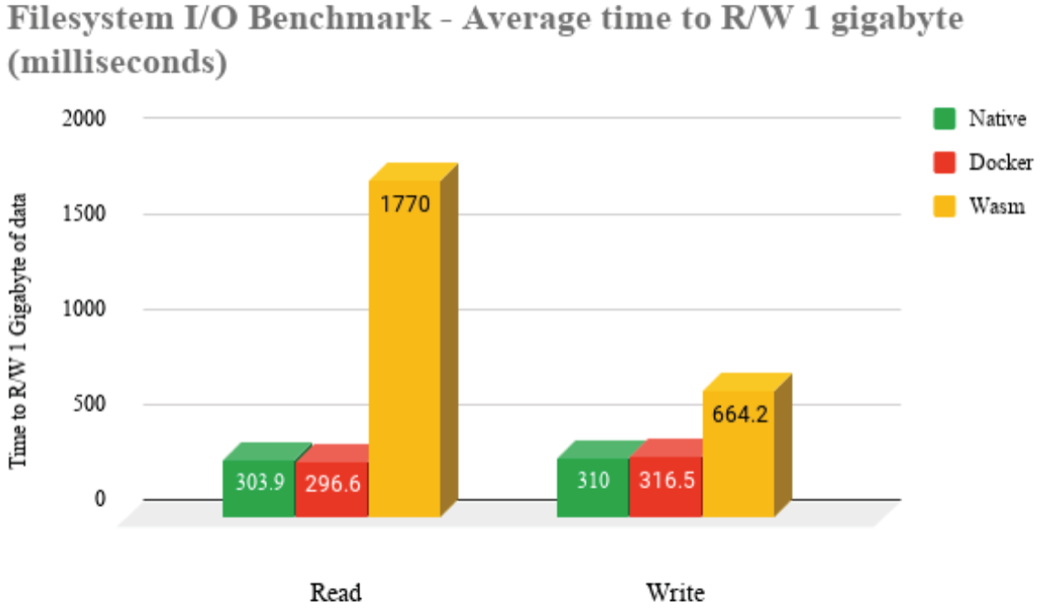
\includegraphics[scale=1]{litr15}
\caption{\footnotesize{Average time to perform I/O Read and Write for 1 (one) gigabyte of data between WebAssembly, Docker and Native applications \cite{lit29}}}
\captionsetup{aboveskip=0pt,font=it}
\end{figure}
\bigskip

Serverless technology was first commercially used in the Amazon Web Service (AWS) lambda application \cite{lit30}. Ever since then, the majority of serverless technology services have been developed and consumed within the cloud computing sector. The biggest selling point of serverless technology is that hardware infrastructures don’t need to be maintained by individual customers. Instead, all the infrastructures are maintained by the company providing the service. For example, Amazon Web Service, Google Cloud Platform (GCP), and Microsoft Azure. Therefore, instead of spending time and money setting up and configuring physical infrastructures, the customer only needs to worry about developing software solutions. When it comes to deploying the software, all they need to do is simply to run a command. The system will then package and deploy the code to the cloud platform in the form of “lambda containers”. Once the code is active in the cloud server, it will be executed on demand when devices send in requests. Therefore, serverless technology is also referred to as “Function-as-a-Service” (FaaS) \cite{lit31}.

Gackstatter (2021) conducted very detailed research and listed a number of questions regarding WebAssembly containers running on IoT and edge devices using serverless technology \cite{lit32}. Gackstatter conducted tests and compared cold start-up time as well as runtime performance on applications running with serverless technology in Docker containers and WebAssembly containers on edge IoT devices, Gackstatter also would like to know if WebAssembly is suitable for edge IoT devices running programs using the serverless technology.

After conducting research and performing comparisons, Gackstatter observed that WebAssembly performed better than Docker on both start-up time and runtime throughput. The author concluded that WebAssembly is able to consume anywhere between 94\% less time on a server machine to 99.5\% less time on a Raspberry Pi than Docker containers when performing a cold start-up. WebAssembly programs also run faster than Docker programs, from 1.6 to 3 times the throughput on a server machine to anywhere between 2.4 and 4.2 times the throughput on a Raspberry Pi.

\bigskip
\begin{figure}[hp]
\centering
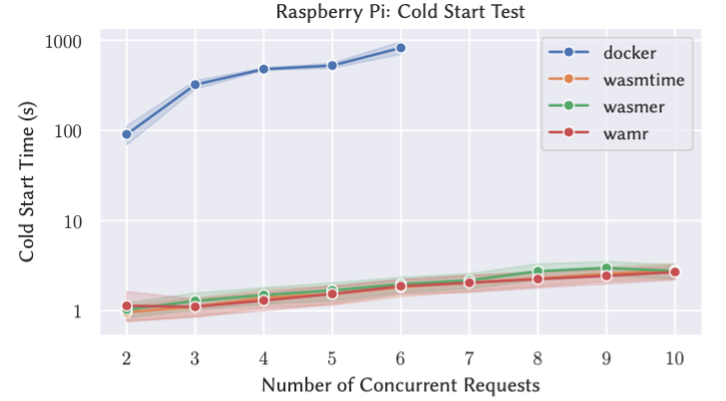
\includegraphics[scale=1]{litr16}
\caption{\footnotesize{Average cold start-up time between Docker container and WebAssembly runtimes (wasmtime, Wasmer, wamr) \cite{lit32}}}
\captionsetup{aboveskip=0pt,font=it}
\end{figure}
\bigskip

In conclusion, Gackstatter found that WebAssembly is very suitable for serverless technology. Some of the main supporting arguments presented were that WebAssembly is able to be compiled from multiple languages, such as C, C++, and Rust with more language compilers currently under development. Furthermore, from the aforementioned time compression, WebAssembly with serverless has an unprecedented lead over Docker container on cold start-up time and throughput.

\bigskip
\section{New Ideas and Beyond}

Gadepalli et al. (2020) from The George Washington University and Arm Research developed and presented a new WebAssembly runtime – aWsm alongside a new WASM serverless framework – Sledge \cite{lit33} \cite{lit34}.

\newpage
\bigskip
\begin{figure}[hp]
\centering
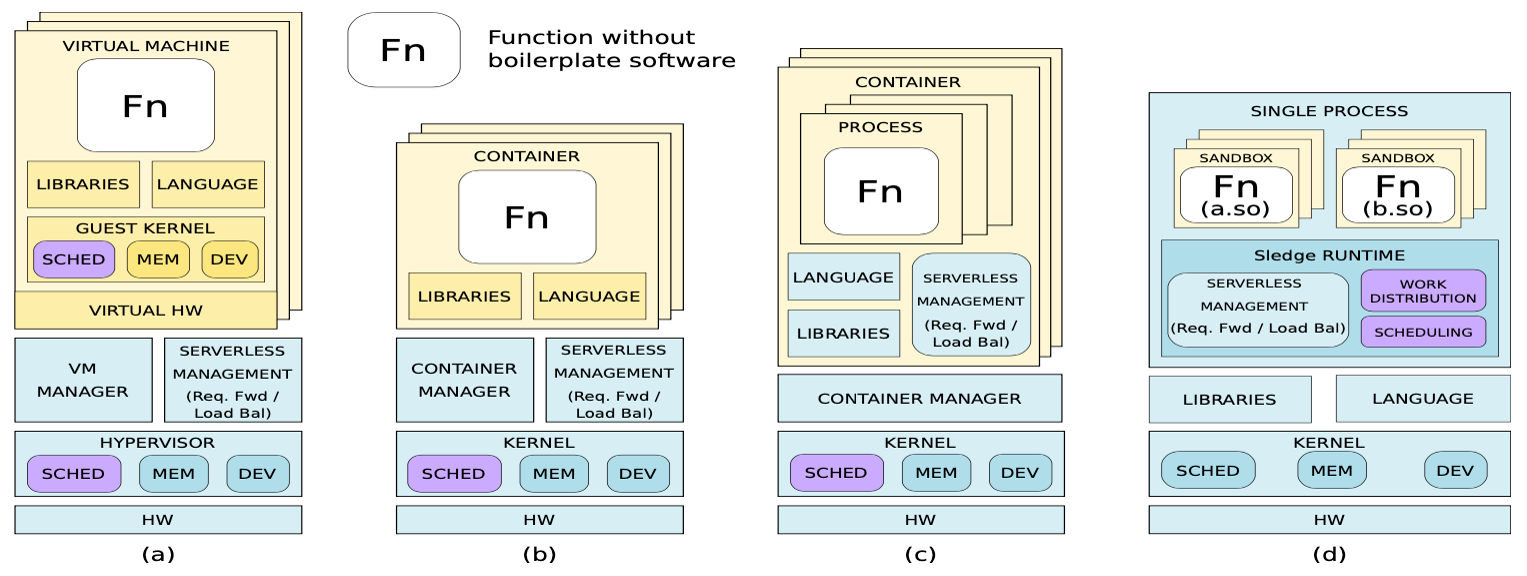
\includegraphics[scale=1]{litr17}
\caption{\footnotesize{Different methods to run applications with serverless technology. The Sledge frame uses the “d” solution \cite{lit34}}}
\captionsetup{aboveskip=0pt,font=it}
\end{figure}
\bigskip

According to the authors, almost all edge IoT devices require low latency and near real-time data processing technology. Gadepalli et al. believe that the lightweight feature of WebAssembly can be optimised for serverless IoT frameworks to achieve low start-up times. And for IoT and edge devices, the ability to perform event-driven, short-lived functions with near real-time, low-latency data processing time is essential. The main competitor of Sledge is Nuclio \cite{lit35}, which is a non-WebAssembly serverless framework that relies on Docker and Kubernetes \cite{lit36}. Just like Sledge, Nuclio is also designed to run on IoT and edge devices.

In \cite{lit33}, Gadepalli et al. developed a new WebAssembly runtime called aWsm (pronounced as “awesome”). aWsm is a very efficient WebAssembly runtime that focuses on solving the “cold-start” issue on serverless containers. It has a “hot swap” feature that only require serverless containers to start once at the very beginning – usually when the device is turned on. From the table below, we can see that the start-up times with aWsm implemented are significantly lower compared to the initial cold-start time.

\begin{figure}[hp]
\centering
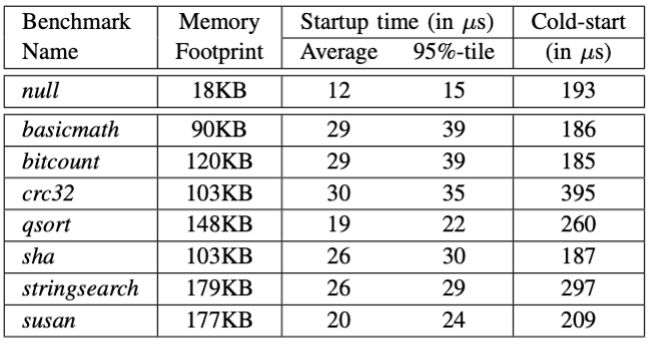
\includegraphics[scale=0.6]{litr18}
\caption{\footnotesize{Start-up time and cold-start time on benchmark programs executed using the aWsm runtime \cite{lit33}}}
\captionsetup{aboveskip=0pt,font=it}
\end{figure}

The biggest feature of Sledge is that combined with aWsm, it is able to perform “hot-swap” while the serverless containers are running. This feature gives plenty of advantages to Sledge because when executing repetitive tasks, it has the ability to start new programs extremely fast. Thus, avoiding the issue of container cold starts. On the other hand, it can also perform on-device real-time data calculations swiftly due to the lightweight feature of WebAssembly.

The author compared Sledge to its main competitor – Nuclio \cite{lit35}. During the performance test, 5 tasks in total were executed. After running all the tests, the result data was observed and analysed by the researchers. As expected, Sledge was able to run the majority of the programs faster than Nuclio. However, the researchers discovered that when running CPU-intensive programs or functions such as image resizing and license plate detection, Nuclio had a better performance than Sledge.

\bigskip
\begin{figure}[hp]
\centering
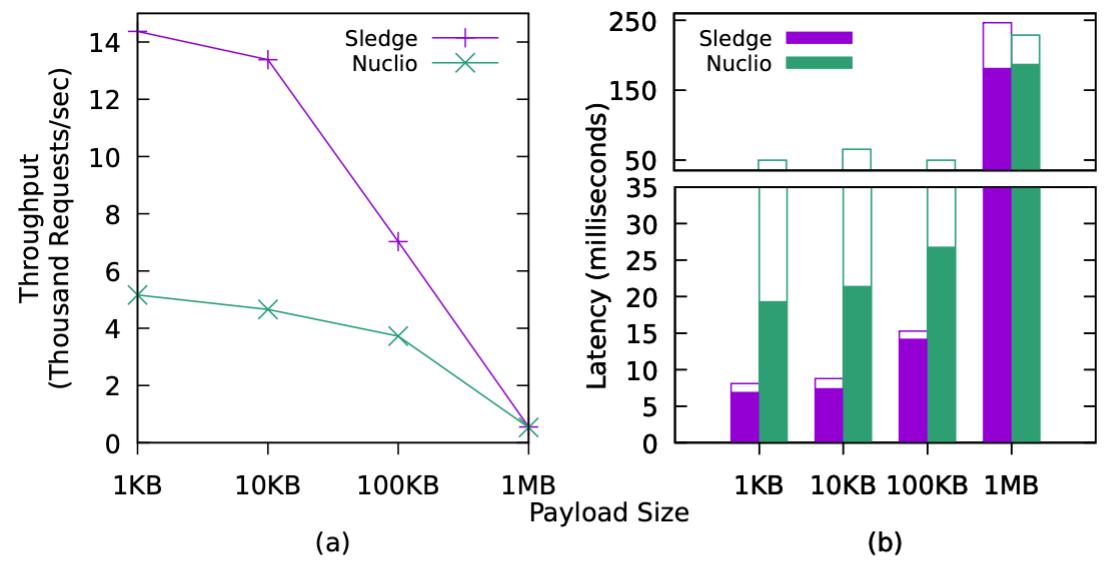
\includegraphics[scale=1]{litr19}
\captionsetup{aboveskip=0pt,font=it}
\end{figure}
\newpage
\begin{figure}[hp]
\centering
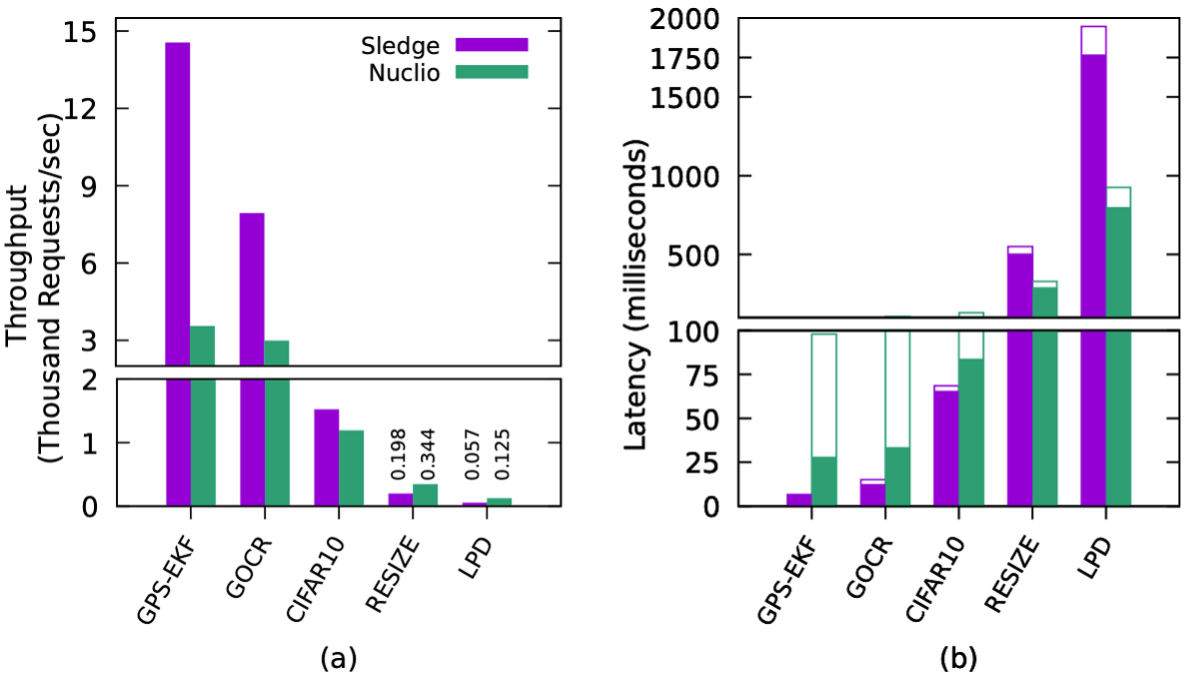
\includegraphics[scale=1]{litr20}
\caption{\footnotesize{The performance comparison between the two frameworks during the payload test and the CPU applications test \cite{lit34}}}
\captionsetup{aboveskip=0pt,font=it}
\end{figure}
\bigskip

At the same time, developers and researchers have built other software that solves critical issues for applications running on the edge network. Nieke et al. designed and developed Edgedancer, a platform that provides support and security to the infrastructure and migration for applications running on the edge \cite{lit37}. Edgedancer allows clients to migrate their mobile web servers between different PaaS (Platform as a service) providers for different needs and scenarios, thus preventing a particular cloud PaaS vendor from having all the control over the client’s data and the web application itself.

Nieke et al. realise and recognise the “lock-in” issue from PaaS cloud providers. The authors stated that currently, it is a tedious and difficult process for mobile application service providers to relocate and migrate their software infrastructure and deployment from one PaaS provider to another. And this is by design from the cloud vendors. This way, it is more likely for clients to keep using the service provided by one particular cloud vendor, potentially costing the clients’ money and losing out on better or newer services provided by other cloud vendors. Seeing this, Nieke et al. proposed and envisioned a new standard for running web servers in the cloud. Edgedancer is designed to act as the “middle layer” between the server application and the PaaS cloud platform. Edgedancer can run on either clients’ own server machines or hosted in the cloud running remotely. It aims to enable 6 essential features. They are 1 – Server application will be able to migrate between different platforms while it is running with minimum downtime, 2 – Feature 1 can be performed on any devices regardless of the hardware architecture, 3 – Being able to work with applications that are written in any languages, 4 – The relocation and the migration process should be done swiftly, again to achieve minimum downtime, 5 – The host server that is hosting the software need to be protected from any potentially malicious code in the hosted applications, and finally 6 – The opposite from feature 5, applications hosted on the server with the software need to be protected from malicious code on the server itself.

Edgedancer provides a few migration configurations. They are Platform controlled, Agent controlled, and Hybrid migration. Platform controlled essentially controls the migration process based on the parameters the client has set, including the time, the condition and the migration target. In the Agent controlled mode, the client has full control of the time and the target of migration. For example, a gaming platform might want to migrate their server to a high-performance, low-latency server for a few hours in order to host special in-game events, then migrate the server back for normal usage. Lastly, Hybrid migration is a mixture of both.

The author developed the software with the help of WebAssembly largely because of the “sandbox” model WebAssembly provides when running applications on native devices. During earlier reviews, we mentioned several benefits “sandbox” can provide. Specifically, this gives Edgedancer an excellent out-of-the-box security foundation. On top of that, Edgedancer can be run using any WebAssembly runtimes, namely WAMR, Wasmtime, or Wasmer.

\bigskip
\begin{figure}[hp]
\centering
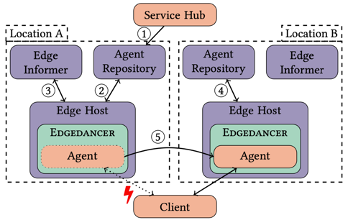
\includegraphics[scale=0.7]{litr21}
\caption{\footnotesize{The design architecture of Edgedancer \cite{lit37}}}
\captionsetup{aboveskip=0pt,font=it}
\end{figure}
\bigskip

\bigskip
\section{Put into Practice}

After all the proposals, solutions and evaluations from the research articles we have reviewed so far, we would like to know what it looks like to apply the technologies to real-world applications.

Pelle et al. undertook research and experiments to move edge technology into cloud computing. Enabling all applications currently running on the cloud to also run on the edge \cite{lit38}. Particularly, instead of blindly applying the edge technology to the current cloud infrastructure hosted on AWS or Google Cloud Platform, the authors designed and developed a new middleware solution that runs on top of the current infrastructure layers. Thus, simplifying the steps needed to integrate and migrate current cloud applications to run on the edge.

The authors identified an area that suits well with this technology, namely, object detection during HD video streaming. They argue that using WebAssembly to exchange and encode/decode video data reduces the backend processing time significantly. Thus, enabling a faster connection and processing time to create a better streaming experience for the client users.

The authors then designed and developed an implementation of the software. They used Python with the OpenCV library for image processing and object detection \cite{lit39}. The software was then deployed to Amazon Web Service Greengrass which is an IoT/edge runtime and hosting service \cite{lit40}.

\begin{figure}[hp]
\centering
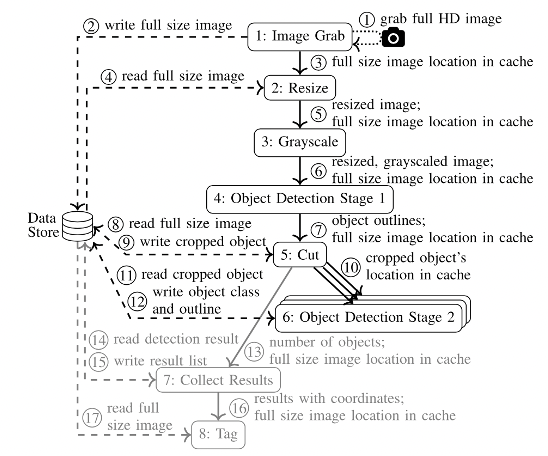
\includegraphics[scale=0.5]{litr22}
\caption{\footnotesize{Design flow chart for video object detection software implementation \cite{lit38}}}
\captionsetup{aboveskip=0pt,font=it}
\end{figure}
\bigskip

During the benchmarking, the authors found the performance of the software running on the edge outperformed the software distributed on the cloud consistently across all functions. Therefore, the initial theory formed by the authors has been proven and the middleware application they developed indeed performed as expected.

\bigskip
\begin{figure}[hp]
\centering
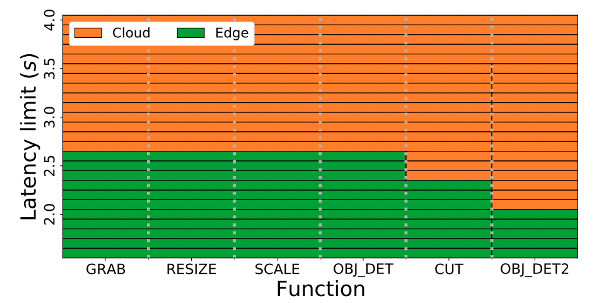
\includegraphics[scale=0.6]{litr23}
\caption{\footnotesize{Performance for each function between cloud-based implementation and edge-based solution \cite{lit38}}}
\captionsetup{aboveskip=0pt,font=it}
\end{figure}
\bigskip

The authors did not specify any further research questions. However, the team has proposed and is currently looking into adding an additional optimisation component on top of the layers to achieve even better performance and lower latencies.

On the other hand, Xu et al. performed comprehensive research and study into developing, deploying and benchmarking the performance of an edge framework running on a public edge platform. As well as comparing the recorded performance with a few current solutions. According to the authors, this research is a first-of-its-kind study within the field \cite{lit41}.

The authors mainly performed this study from the end users’ and the edge providers’ perspectives. In this context, end users represent the users who deploy their apps on the platform; edge providers refer to the company that runs and maintains those platforms. Xu et al. chose Alibaba ENS to be the testing edge provider \cite{lit42}, to compare with Microsoft Azure. They collected the performance data and the workload data from both deployments. Specifically, they first conducted tests to collect benchmark data such as latency and throughput before deploying custom-made applications to both platforms to simulate a real-world scenario.

The authors found that under Wi-Fi, LTE (4G) and 5G internet connections, the edge platform consistently outperforms the traditional cloud platform across all connection methods with a much lower RTT (round trip time). Specifically, under Wi-Fi connection, RTT for the connection to the nearest edge site is 1.89 times faster than to the nearest cloud site. Even more, it is 3.4 times faster than to the average cloud site.

\bigskip
\begin{figure}[hp]
\centering
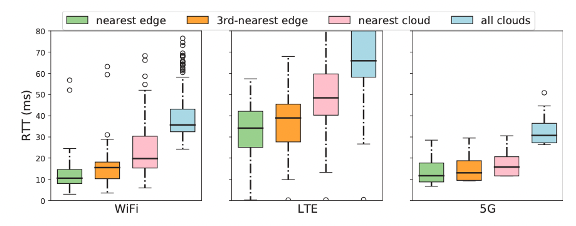
\includegraphics[scale=0.7]{litr24}
\caption{\footnotesize{The Medium RTT (round-trip-time) for deployment implementations \cite{lit41}}}
\captionsetup{aboveskip=0pt,font=it}
\end{figure}
\bigskip

After that, they performed and measured the throughput between the cloud platform and the edge platform. They found that with throughput, it is a lot more difficult to get an accurate reading because throughput data is dictated by multiple factors. For example, under LTE and 5G connections, there is a bottleneck on the uplink bandwidth, and with Wi-Fi connections, throughput is also capped by the wireless router’s bandwidth. The authors argue that only when throughput is extremely high or the distance between client and site is extremely far, we will then observe a significant difference between the raw throughput between the edge platform and the cloud platform.

The experiment proves the argument, the difference between cloud platform and edge platform under normal circumstances is negligible (corr < 0.7). However, when the mean throughput is greater than 200 Mbps (megabits per second), then only edge platform will become more efficient than cloud platform. In below figure, we can see that the greater the mean throughput is, the bigger the difference become between cloud platform and edge platform (corr $\geq$ 0.7).  However, the author stated that there are very few applications require that amount of connection throughput. For example, video streaming at 4K resolution as well as running on 60 FPS (frames per second) only has a throughput of fewer than 100 Mbps.

\bigskip
\begin{figure}[hp]
\centering
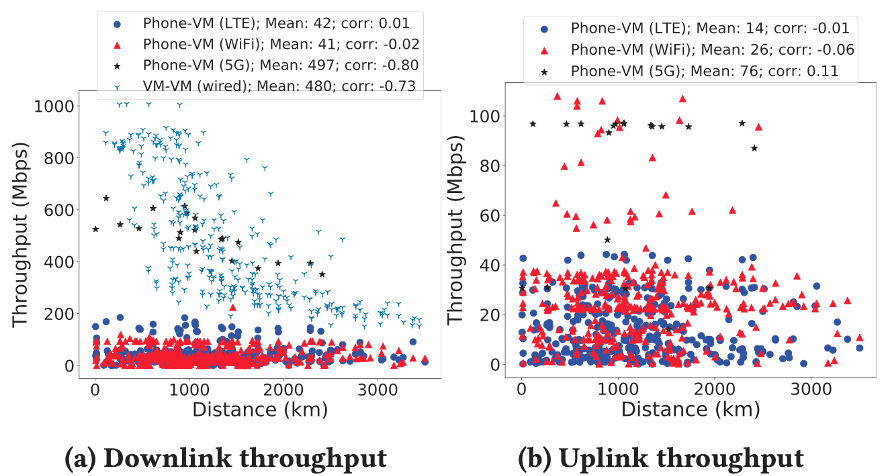
\includegraphics[scale=0.4]{litr25}
\caption{\footnotesize{Downlink (a) and uplink (b) throughput comparison between edge VM and cloud (4G LTE, 5G, Wi-Fi) \cite{lit41}}}
\captionsetup{aboveskip=0pt,font=it}
\end{figure}
\bigskip

Finally, the authors conducted performance testing with the software that represents real-world scenarios. In particular, two kinds of software were used during the experiment, cloud gaming and live video streaming.

After the cloud gaming test, the author discovered that edge platforms indeed performed better with a lower response time than traditional cloud platforms. In fact, all edge implementations were able to achieve a response time around 100ms and below 125ms, while only one device – Samsung Note 10+ running on the optimal cloud environment (short distance between the client’s physical location and the cloud server) can achieve a response time within 100ms. The author concluded that the performance of the edge platform implementation when running cloud gaming is fast enough that it is no longer considered the bottleneck of what’s causing the delay in gaming. Instead, in order to further reduce the response time, there simply need better hardware to render faster thus achieving an even better gaming experience.

\newpage
\begin{figure}[hp]
\centering
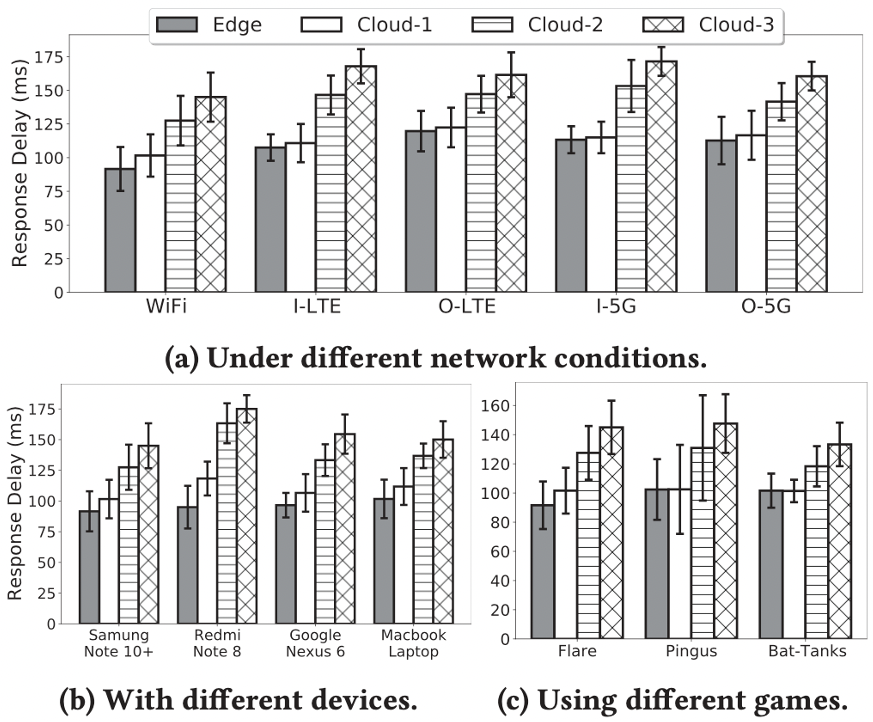
\includegraphics[scale=0.3]{litr26}
\caption{\footnotesize{Cloud gaming performance with different platforms (a), devices (b) and game types (c) \cite{lit41}}}
\captionsetup{aboveskip=0pt,font=it}
\end{figure}

Similar to the throughput experiment, the authors discovered that the performance difference on streaming delays between edge platform and cloud platform is also negligible because of a number of other factors also impacting the time delay on video streaming. For example, image capture, transcoding, software configuration and so on. However, in terms of the result data, edge platform still came on top with an average increase of 24\% compared to the fastest 5G cloud platform. The authors suggested instead of pursuing faster network connections, streaming video on devices with more computational power as well as appropriately configured streaming software will have more effect on the video streaming experience.

\begin{figure}[hp]
\centering
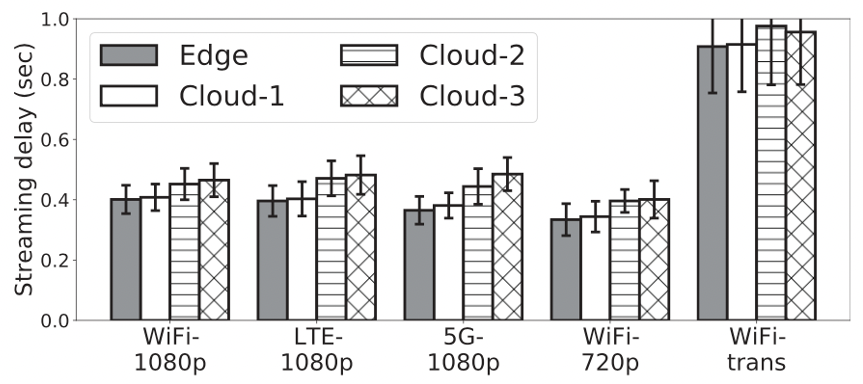
\includegraphics[scale=0.3]{litr27}
\caption{\footnotesize{Video streaming delays between edge and cloud under different network environments \cite{lit41}}}
\captionsetup{aboveskip=0pt,font=it}
\end{figure}
\bigskip

In the end, the authors concluded that the main reason for companies and developers to migrate and adapt their current software systems to edge platforms is for monetary reasons. With less connection time and bandwidth needed due to edge’s efficiency, apps and software deployed on the edge platform are able to reduce their operating cost by up to 98\% on certain applications. On top of that, running on the edge will simply be more efficient with less delay and RTT as well as better throughput, which can be attractive for companies in certain industries. Finally, the authors recognise the fast-growing demand in the edge market, and they predict that more apps and software will be deployed on edge platforms in the upcoming years.

\bigskip
\section{Thorough Review}

Our final literature review is written by Gackstatter et al. (2022) and it is one of the latest and most comprehensive studies conducted in regard to running and benchmarking WebAssembly on the edge \cite{lit43}. In this study, the authors recognise the lengthy start-up time traditional serverless technologies (FaaS) such as Amazon Lambda or Firebase Functions (Google) have \cite{lit30} \cite{lit44}. The authors discovered that 81\% of all functions are invoked less than once per minute and 50\% of them execute for less than 1 second on Microsoft Azure. This means it is very likely that it actually takes longer to start up and shut down the container than to execute the function itself, thus costing extra time and energy.

Gackstatter et al. developed WOW - A WebAssembly container runtime for OpenWhisk, to tackle the serverless cold start problem in Apache OpenWhisk \cite{lit45}. In fact, in 2021, Gackstatter has already conducted benchmarking experiments with various existing runtimes and frameworks \cite{lit32}. During the research in 2021, Gackstatter discovered that running WebAssembly containers rather than Docker containers on OpenWhisk can increase cold start-up time by 99.5\%.

WOW is designed to be run as a middleware on top of OpenWhisk. First of all, it is written in Rust which is itself a high-performance low-level language. Furthermore, WOW uses an island module design managed by a dynamic HashMap to look up and store data instantaneously. It interacts with OpenWhisk as well as client applications using JavaScript Object Notation (JSON).

\newpage
\bigskip
\begin{figure}[hp]
\centering
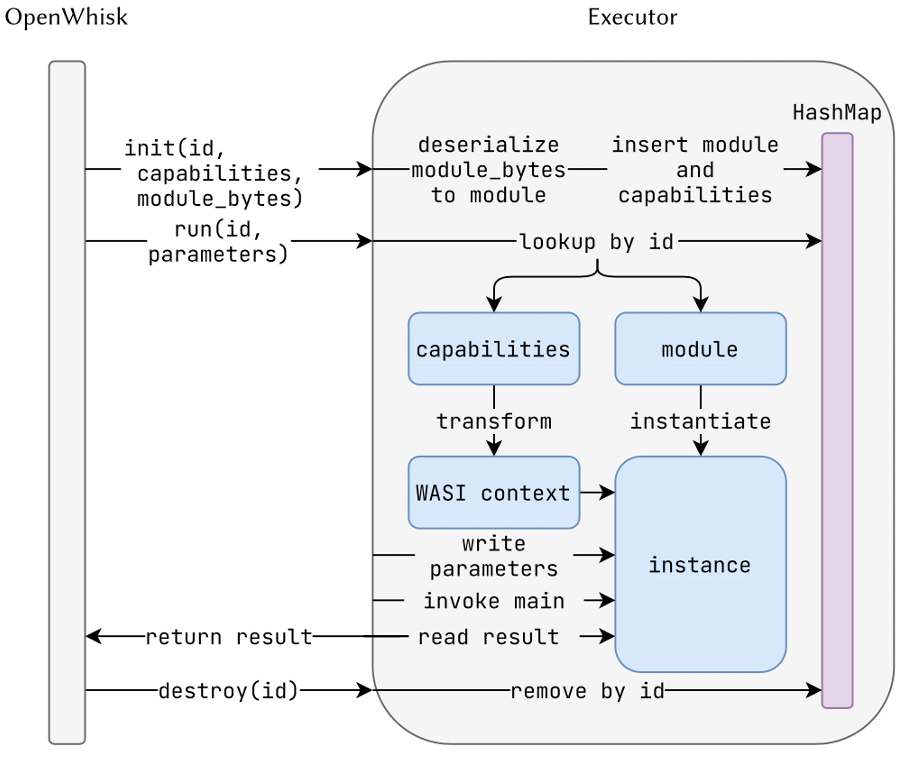
\includegraphics[scale=0.4]{litr28}
\caption{\footnotesize{Visualisation of WOW’s design \cite{lit43}}}
\captionsetup{aboveskip=0pt,font=it}
\end{figure}
\bigskip

There are also dramatic improvements in terms of throughput and latency for WOW implementations compared to Docker containers. WOW achieves on average 3.5 times more throughput than Docker containers. It also reduces the latency by 99.5\% on average and uses 5.6 times less memory than Docker containers on average, which are very considerable improvements.

From the above literature reviews, we have observed and learned a lot within the field of WebAssembly, including what other researchers are working on as well as the latest technology currently under development. From here, we will be able to design and conduct our own research and experiment to further understand and to elaborate on the questions within this field, and to contribute to the industry by producing and showcasing the results from our own works.